\documentclass[11pt,letterpaper]{article}
\usepackage{cogsys}
\usepackage[T1]{fontenc}
\usepackage{times}
\usepackage{graphicx}
\usepackage{booktabs}
\usepackage{amsmath}
\renewcommand{\thetable}{S\arabic{table}}
\renewcommand{\thefigure}{S\arabic{figure}}
\newcommand{\trellis}{\textsc{Trellis}}

\cogsysheading{X}{2026}{1-26}{12/2026}{X/2027}
\ShortHeadings{Supplement: Concepts and Chunks from Raw Experience}{K.\ Singaravadivelan and P.\ Langley}

\begin{document}
\raggedbottom

\title{Supplementary Material for ``Learning Concepts and Chunks from Raw Experience''}

\author{Karthik Singaravadivelan}{ksingara3@gatech.edu}
\author{Pat Langley}{patrick.w.langley@gmail.com}
\address{Georgia Institute of Technology, Atlanta, GA 30332 USA; \
         Institute for the Study of Learning and Expertise,
         2164 Staunton Court, Palo Alto, CA 94306 USA}


This document holds the tables and figures that the main paper cites by number (Tables S1 to S21 and Figures S1 to S7).
Configurations C1 to C11 are those of Table 11 in the main paper. Every result uses TinyStories sentences of three to eight words from a 250-word vocabulary, or Lichess positions, as in the main paper.
Judge 2 is the ensemble of Qwen3-8B and phi-4 that the main paper reports, and the earlier judge is Qwen2.5-3B with a grammaticality probability above .5.

\section{Generation}

\paragraph{Earlier judge.} Table~\ref{tab:genold} gives the fair count under the earlier judge, which chose every setting of the generation study.
Under it \trellis{} beat the GPT on 8 of 8 seeds at 250 and 500 sentences. Judge 2 re-scores the same draws, and Table~\ref{tab:agree} gives the agreement between the two judges on the distinct new sentences.
The judges disagree on about one fifth of the sentences, and 77 to 83\% of the disagreements are sentences that judge 2 passes and the earlier judge rejects.
The pass-rate shift is similar across the three models (+.08 to +.15) and largest for the GPT at 4,000 sentences (.66 to .81). Because the GPT also writes more distinct sentences per draw, its fair count rises more than that of \trellis{} under judge 2 at 250 and 500 sentences (+.076 and +.098 against +.061 and +.074).
Judge 2 passes a single adjacent swap in .13 of cases, so its counts are somewhat inflated for every model.

\begin{table}[h]
\caption{Fair count on TinyStories sentences with the Qwen2.5-3B judge (configuration C1). Top: mean over eight seeds with paired differences (mean, 95\% $t$ interval, seeds won).
Bottom: the four confirmation seeds 29, 31, 37, and 41, which chose no setting, with paired differences (mean, 95\% bootstrap interval, seeds won). The 4,000-sentence row uses seeds 13 and 17.}
\label{tab:genold}
\begin{center}
\footnotesize
\begin{tabular}{rcccll}
\toprule
$n$ & \trellis{} & LSTM & GPT & \trellis{} $-$ LSTM & \trellis{} $-$ GPT \\
\midrule
\multicolumn{6}{l}{\textit{All eight seeds}} \\
250   & .242 & .232 & .207 & +.010 [$-$.011, +.030], 5/8 & +.035 [+.016, +.054], 8/8 \\
500   & .298 & .299 & .274 & $-$.001 [$-$.013, +.011], 4/8 & +.024 [+.010, +.039], 8/8 \\
1,000 & .328 & .335 & .328 & $-$.007 [$-$.028, +.015], 3/8 & $-$.000 [$-$.023, +.022], 4/8 \\
4,000 & .319 & .358 & .362 & $-$.039, 0/2 & $-$.043, 0/2 \\
\midrule
\multicolumn{6}{l}{\textit{Four confirmation seeds}} \\
250   & .243 & .221 & .201 & +.022 [$-$.001, +.040], 3/4 & +.042 [+.018, +.069], 4/4 \\
500   & .295 & .294 & .265 & +.002 [$-$.006, +.011], 2/4 & +.030 [+.013, +.052], 4/4 \\
1,000 & .318 & .325 & .332 & $-$.007 [$-$.029, +.019], 1/4 & $-$.014 [$-$.027, $-$.001], 1/4 \\
\bottomrule
\end{tabular}
\end{center}
\end{table}

\begin{table}[h]
\caption{Agreement between the Qwen2.5-3B judge (probability above .5) and judge 2 (Qwen3-8B and phi-4 syntax pass) on all distinct new sentences that \trellis{}, the LSTM, and the GPT generated at the configuration C1 settings on TinyStories, pooled over eight seeds (two seeds at 4,000 sentences).}
\label{tab:agree}
\begin{center}
\small
\begin{tabular}{rccccc}
\toprule
$n$ & Sentences & Agreement & Kappa & Pass rate, earlier judge & Pass rate, judge 2 \\
\midrule
250 & 25,391 & .808 & .617 & .411 & .513 \\
500 & 29,942 & .805 & .614 & .467 & .580 \\
1,000 & 31,223 & .801 & .586 & .555 & .677 \\
4,000 & 8,953 & .790 & .547 & .581 & .720 \\
\bottomrule
\end{tabular}
\end{center}
\end{table}

\paragraph{Boundary-strict count.} Table~\ref{tab:strict} gives the boundary-strict count under the earlier judge from the eight-seed run. The strict count drops distinct sentences whose first word never starts, or whose last word never ends, a real held-out sentence, for every model alike.
Under it \trellis{} matches the LSTM and beats the GPT only at 250 sentences, and at 1,000 sentences it trails both by about .014.
A match requires a paired interval that includes zero with a lower bound above $-.03$. Under the $t$ interval, \trellis{} matches the LSTM at 500 sentences on the strict count, and the bootstrap interval says otherwise.

\begin{table}[h]
\caption{Boundary-strict fair count on TinyStories (configuration C1, Qwen2.5-3B judge), mean over eight seeds, with paired differences (mean, 95\% $t$ interval, seeds won).}
\label{tab:strict}
\begin{center}
\footnotesize
\begin{tabular}{rcccll}
\toprule
$n$ & \trellis{} & LSTM & GPT & \trellis{} $-$ LSTM & \trellis{} $-$ GPT \\
\midrule
250   & .224 & .215 & .196 & +.008 [$-$.010, +.027], 5/8 & +.028 [+.010, +.045], 7/8 \\
500   & .273 & .282 & .262 & $-$.009 [$-$.021, +.002], 2/8 & +.011 [$-$.006, +.027], 5/8 \\
1,000 & .300 & .315 & .314 & $-$.014 [$-$.039, +.010], 2/8 & $-$.014 [$-$.036, +.009], 2/8 \\
\bottomrule
\end{tabular}
\end{center}
\end{table}

An earlier four-seed run under the earlier judge found a GPT deficit of .014 at 1,000 sentences, and the four additional seeds did not replicate it.
The temperature grid for \trellis{} extended past the neural grids after its optimum at 250 sentences sat on the grid edge, while the neural optima were interior. At 250 sentences the optimum later moved to temperatures of 4.0 to 4.5, and the main paper reports the pre-fixed value 3.5.
The four selection seeds supplied the pre-fixed setting for the eight-seed comparison.
The earlier judge passes about .89 of real held-out sentences, so no generator can exceed that grammaticality rate under it.

\paragraph{Neural baselines.} For each seed and size we chose the size of a neural model by held-out loss on sentences from stories that the stream never reached.
The grid covers 1, 2, or 4 layers, widths 64, 128, or 256, and dropout .1 or .3 for the GPT, and 1 or 2 layers, widths 128 or 256, and the same dropout for the LSTM.
Training uses AdamW with early stopping (patience six, at most 80 epochs). The generation runs recorded no parameter counts. The compression runs retrained the same grid and selected networks of 0.2 to 1.2 million parameters for the LSTM and 0.23 to 1.7 million for the GPT.
We sample each neural model at a tuned temperature, because at low temperature a neural model repeats its training data (2 to 14\% of draws are distinct at temperatures .1 to .3).

\paragraph{Judge agreement.} Judge 2 passes more generated sentences than the earlier judge does (.51 to .72 against .41 to .58 of distinct new sentences). The two judges agree on 79 to 81\% of sentences (kappa .55 to .62), and nearly all disagreements are sentences that judge 2 passes and the earlier judge rejects.

\paragraph{Frontier of novelty and grammaticality.} A model that copies its training data writes grammatical sentences that are all stored, whereas a model that recombines parts freely writes new sentences and makes more errors.
To compare models at matched novelty we measure the share of new distinct sentences that contain a trigram unseen in training. Table~\ref{tab:novel} and Figure~\ref{fig:frontier} show that every learner pays for novelty with grammaticality.
At about a third novel, \trellis{} with a three-word window is grammatical .76 of the time and the LSTM .92. At about half novel the LSTM and GPT reach .81 and .80, whereas \trellis{} with windows of four and five words reaches .71 and .67.
Shorter windows copy more, and longer windows generalize more and err more. These runs use the plain generator (configuration C2, without the exact-boundary rule).

\begin{figure}[!t]
\centering
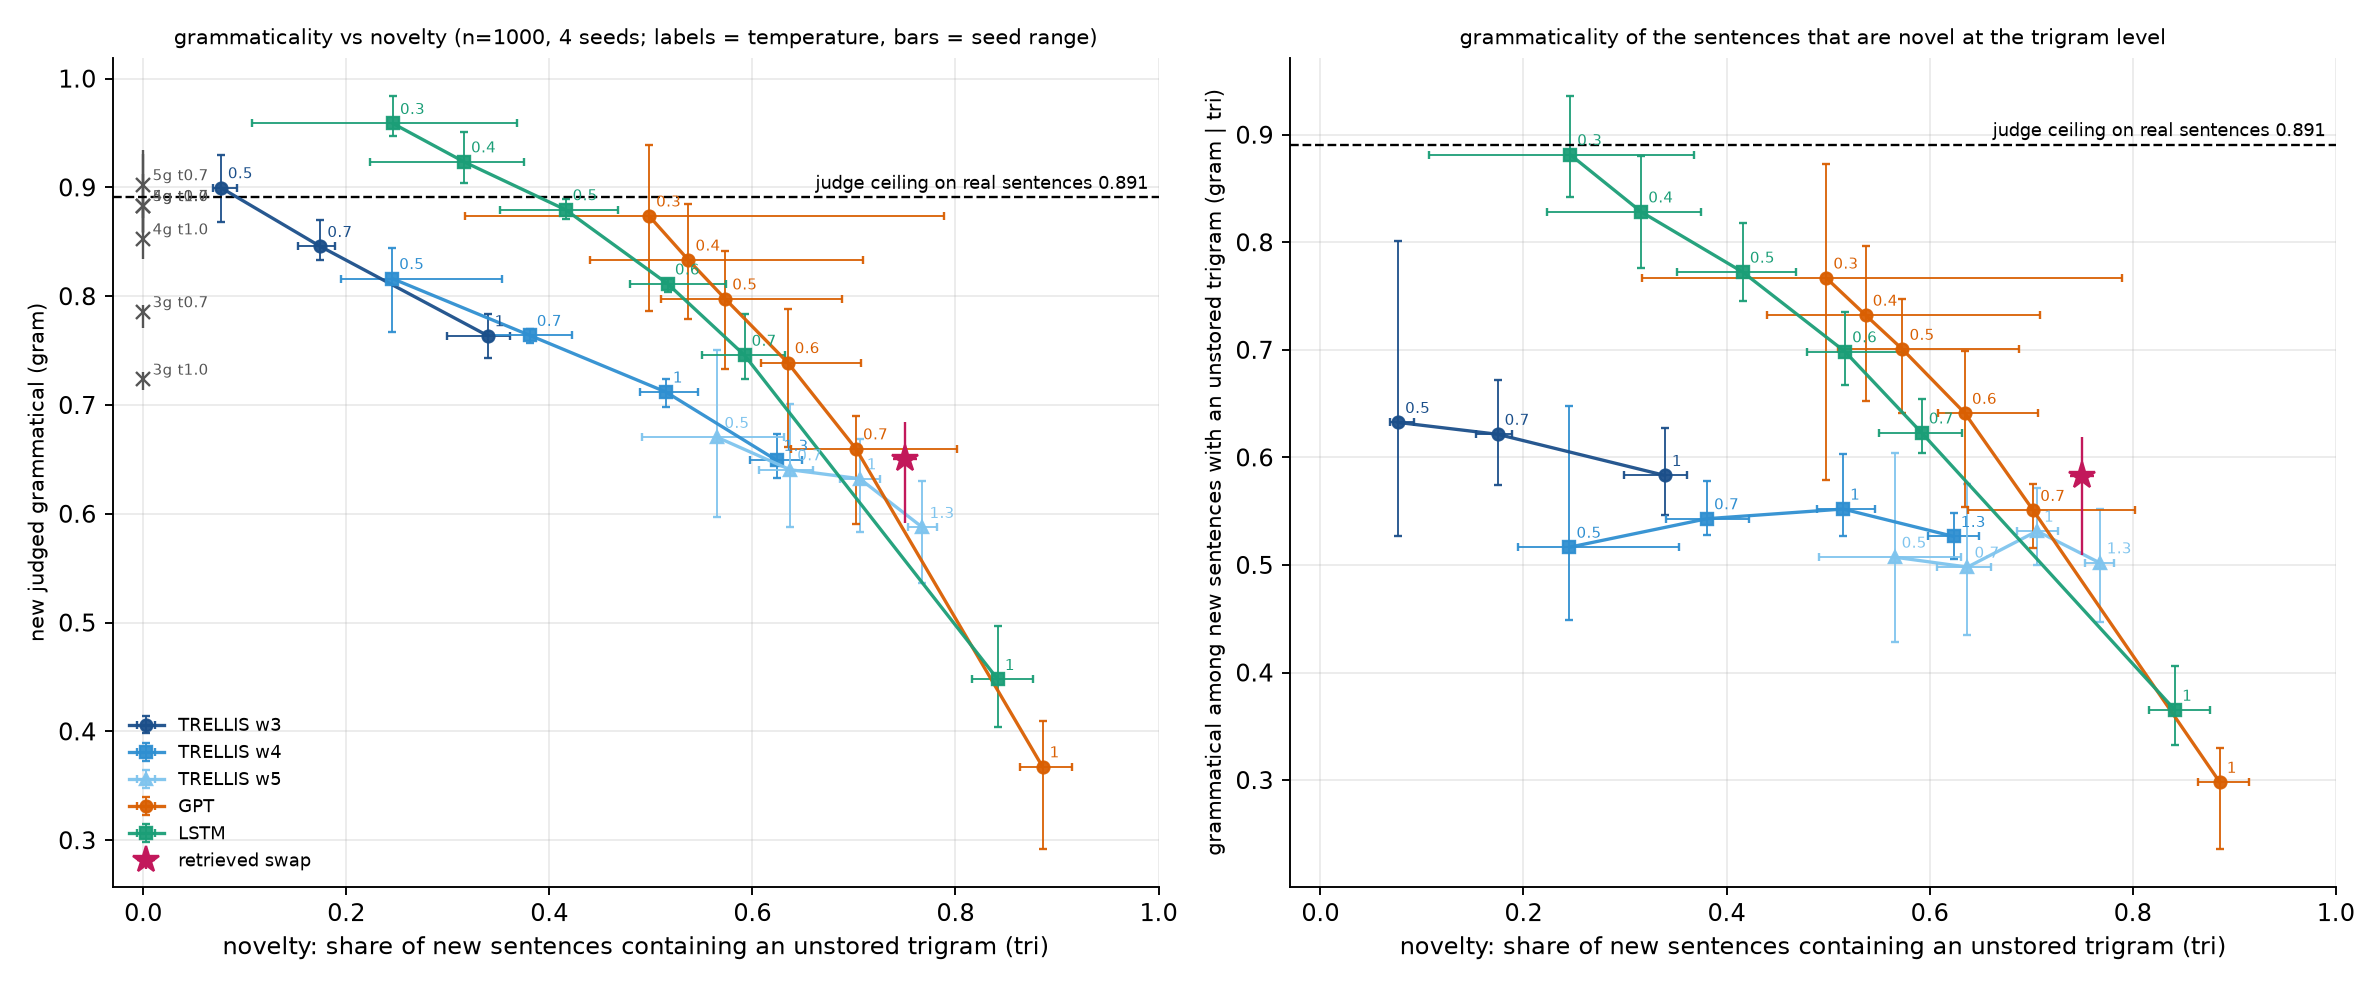
\includegraphics[width=\textwidth]{figures/story_frontier}
\caption{Grammaticality against novelty after 1,000 TinyStories sentences (four seeds; labels give sampling temperature, bars give the seed range; Qwen2.5-3B judge; configuration C2).
Novelty is the share of new distinct sentences containing a trigram unseen in training. Left, share of new sentences judged grammatical; right, grammaticality among the sentences that are novel at the trigram level.
The dashed line marks the judge's pass rate on real sentences (.891). Models: \trellis{} with windows of 3, 4, and 5 words, GPT, LSTM, and a reference generator that swaps one word in a retrieved training sentence (star).}
\label{fig:frontier}
\end{figure}

\begin{table}[h]
\caption{Share of new distinct sentences with a trigram unseen in training (new trigram) and share judged grammatical at matched novelty, after 1,000 TinyStories sentences (four seeds, Qwen2.5-3B judge, configuration C2).
The judge passes .89 of real held-out sentences. Each row is the setting whose novelty matches its partner.}
\label{tab:novel}
\begin{center}
\small
\begin{tabular}{lcc}
\toprule
Model & New trigram & Grammatical \\
\midrule
\trellis{}, window 3 & .34 & .76 \\
LSTM & .32 & .92 \\
\trellis{}, window 4 & .52 & .71 \\
LSTM & .52 & .81 \\
\trellis{}, window 5 & .57 & .67 \\
GPT & .57 & .80 \\
\bottomrule
\end{tabular}
\end{center}
\end{table}

\paragraph{Where \trellis{} falls behind.} From 1,000 to 4,000 sentences all three models write more distinct sentences, yet only the new-trigram sentences of \trellis{} become less grammatical.
Under the earlier judge the share falls from .484 to .410 for \trellis{}, against .494 to .498 for the LSTM and .471 to .570 for the GPT (eight seeds at 1,000 sentences, two at 4,000).
Under judge 2 the share that passes syntax falls from .604 to .535 for \trellis{} and rises from .620 to .657 for the LSTM and from .614 to .742 for the GPT. The share that passes both questions falls from .381 to .286 for \trellis{} against .419 to .405 for the LSTM and .389 to .479 for the GPT.
Real text and both neural models innovate after a history seen $k$ times at a rate that depends on $k$ alone. \trellis{} innovates too little after rare histories and too much after frequent ones, and the imbalance grows with the amount of data.
This diagnosis is a hypothesis, because the one attempt to correct the imbalance raised novelty without raising the fair count. We estimate that a correction would recover .015 to .03 of fair count, which still leaves \trellis{} short of parity at 4,000 sentences.
Where a constraint of .90 grammaticality can be met, the LSTM keeps more novelty than \trellis{} (share of unstored trigrams .48 against .19). The tie at the fair-count optimum, where every model is .58 to .66 grammatical, fails at the high-grammaticality end.
Judged with Qwen3-8B and phi-4 under a stricter prompt, no generator reaches .95 grammaticality among its distinct new sentences at 1,000 sentences.

\section{Compression}

Table~\ref{tab:bits} gives every code length behind Figure 3 of the main paper, with the standard deviation over the two seeds.
The test sentences are the first 1,000 kept sentences (three to eight words, 250-word vocabulary) of each seed's held-out stories, and the uniform code over 251 outcomes costs 51.4 bits for a sentence of about 5.5 words and the end symbol.
The share of test sentences that also occur in the training stream is .10, .15, .21, .27, and .36 at 250, 500, 1,000, 2,000, and 4,000 sentences.
On the remaining sentences the ranking is unchanged: byte-pair coding costs 40.1 to 35.6 bits, \trellis{} 38.6 to 34.2, the best n-gram 32.6 to 27.5, and the LSTM 32.0 to 24.9.
The escape weight of the \trellis{} code was $10^{-3}$ in 18 of 20 cells and $10^{-4}$ for concepts off at 4,000 sentences.
Per token (words plus end), \trellis{} costs 5.53 bits at 250 sentences and 4.12 at 4,000, the Kneser-Ney trigram 4.70 and 3.37, and the LSTM 4.61 and 3.10.
We selected every free parameter (merge count, escape weight, n-gram order, network size) on a separate 300-sentence development set and nothing on the test sentences.
Removing both the chunks and the concepts gives a shorter code than the full system at every size, so the margin over byte-pair coding belongs to the word-window generator.

\begin{table}[h]
\caption{Held-out code length in bits per sentence on TinyStories (configuration C8; mean and standard deviation over seeds 13 and 17; model cost not charged).}
\label{tab:bits}
\begin{center}
\footnotesize
\begin{tabular}{lccccc}
\toprule
Model & 250 & 500 & 1,000 & 2,000 & 4,000 \\
\midrule
Uniform over 251 & 51.4 & 51.4 & 51.4 & 51.4 & 51.4 \\
Word unigram & 42.6 & 42.3 & 42.1 & 42.0 & 41.9 \\
Byte-pair encoding and unigram code & 38.0 & 35.7 & 33.1 & 31.0 & 28.7 \\
Witten-Bell trigram & 31.3 & 28.5 & 25.7 & 23.8 & 22.2 \\
Kneser-Ney trigram & 30.3 & 27.7 & 25.1 & 23.3 & 21.7 \\
GPT & 30.2 & 27.3 & 24.4 & 22.2 & 20.6 \\
LSTM & 29.8 & 26.5 & 23.5 & 21.5 & 20.0 \\
\trellis{} & 35.7$\pm$0.2 & 33.2$\pm$0.0 & 30.8$\pm$0.3 & 28.7$\pm$0.1 & 26.6$\pm$0.0 \\
\trellis{}, chunks off & 35.5$\pm$0.1 & 33.5$\pm$0.2 & 30.8$\pm$0.1 & 28.7$\pm$0.1 & 26.7$\pm$0.1 \\
\trellis{}, concepts off & 33.8$\pm$0.1 & 31.2$\pm$0.0 & 28.8$\pm$0.2 & 26.9$\pm$0.2 & 24.9$\pm$0.0 \\
\trellis{}, chunks and concepts off & 33.7$\pm$0.1 & 31.1$\pm$0.0 & 28.6$\pm$0.1 & 26.7$\pm$0.2 & 24.7$\pm$0.1 \\
\bottomrule
\end{tabular}
\end{center}
\end{table}

\section{Parsing}

Full inside-outside cost grows cubically with sentence length, so we tested a spectrum between greedy parsing and full inside-outside at 1,000 sentences (four seeds, configuration C4, set C).
A window variant runs inside-outside inside a window of $W$ symbols, freezes the best parse of its first $S$ symbols, and moves on. A capped variant limits chunks to $2^D$ symbols per pass.
Table~\ref{tab:window} gives selected cells. The sentences have at most eight tokens, so the cost saving here is modest (about a factor of two for the cap-four chart) and grows with length.
Disjoint windows hurt, because a chunk can never cross a window boundary in the pass that creates it, whereas overlapping windows that commit only the first part of the window recover full-parser accuracy against the shallow-phrase reference.
No variant changes acceptance of broken sentences by more than seed noise, so these scores cannot discriminate between parsers. The main paper keeps full inside-outside, and no experiment here measures the cap-four gain on long sentences.
Beam-one greedy parsing matches full inside-outside in F1 against the reference (.353 against .352) and in AUC for ungrammatical sentences (.541 against .542). Of its trees, 93\% are identical to the full ones, and it costs .21 as much.

\begin{table}[h]
\caption{Windowed and capped inside-outside parsing on TinyStories after 1,000 sentences (configuration C4, set C, mean over four seeds). Cost is composites evaluated per sentence relative to full parsing; F1 is against the NLTK shallow-phrase reference
(right-branching scores .423 on the same sentences); ``same as full'' is F1 between the variant's trees and full-parse trees.}
\label{tab:window}
\begin{center}
\small
\begin{tabular}{lcccc}
\toprule
Variant & Cost & F1 vs.\ reference & Same as full & Mean AUC, ungrammatical \\
\midrule
Full inside-outside & 1.00 & .352 & 1.00 & .542 \\
Greedy (beam 1) & .21 & .353 & .934 & .541 \\
Cap-four chart & .53 & .362 & .970 & .542 \\
Window 4, stride 2 & .48 & .413 & .799 & .540 \\
Window 3, stride 2 & .30 & .428 & .788 & .538 \\
Window 4, disjoint & .31 & .308 & .854 & .541 \\
Window 3, disjoint & .21 & .242 & .557 & .558 \\
\bottomrule
\end{tabular}
\end{center}
\end{table}

Two scores come from the memory. The parse score is the inside-pass log probability of the sentence per word, and the generator score is the per-word log probability that the pair-gated generator assigns to each word given its left context.
Table~\ref{tab:parse} gives the share of broken sentences that each score accepts, and Table~\ref{tab:auc} gives the area under the curve (AUC) with which each score separates real held-out sentences from each broken class, at 125 and 4,000 sentences.
The generator score keeps pace with the baselines on scrambles at 125 sentences and trails them at 4,000, and its content-swap AUC at 4,000 sentences is .81 against .88 to .89 for the n-gram, LSTM, and GPT. The parse score is near chance on every class.

\begin{table}[h]
\caption{Share of broken held-out TinyStories sentences accepted by each score (configuration C4, set C, four seeds). The threshold accepts 90\% of 400 real calibration sentences, so lower is better.
\trellis{} parse is the inside-pass log probability per word, \trellis{} generator is the per-word log probability of the pair-gated generator, and LSTM and GPT train on the same sentences.
Every score accepts .89 to .94 of real sentences.}
\label{tab:parse}
\begin{center}
\small
\begin{tabular}{llcccc}
\toprule
Broken class & Score & 125 & 500 & 1,000 & 4,000 \\
\midrule
Scrambled & \trellis{} parse & .88 & .81 & .78 & .77 \\
 & \trellis{} generator & .39 & .19 & .13 & .05 \\
 & LSTM / GPT & .65 / .40 & .16 / .09 & .08 / .04 & .01 / .01 \\
Adjacent swap & \trellis{} parse & .89 & .88 & .87 & .87 \\
 & \trellis{} generator & .75 & .69 & .64 & .53 \\
 & LSTM / GPT & .86 / .78 & .76 / .66 & .69 / .55 & .36 / .20 \\
Content swapped & \trellis{} parse & .94 & .93 & .92 & .91 \\
 & \trellis{} generator & .86 & .79 & .71 & .58 \\
 & LSTM / GPT & .80 / .80 & .66 / .70 & .62 / .64 & .41 / .40 \\
\bottomrule
\end{tabular}
\end{center}
\end{table}

\begin{table}[h]
\caption{AUC for real versus broken held-out TinyStories sentences (configuration C4, set C, four seeds) for the per-word parse score and generator score of \trellis{} and for the 5-gram, LSTM, and GPT trained on the same sentences.}
\label{tab:auc}
\begin{center}
\small
\begin{tabular}{lcccc}
\toprule
Score & \multicolumn{2}{c}{125 sentences} & \multicolumn{2}{c}{4,000 sentences} \\
 & Scramble & Content swap & Scramble & Content swap \\
\midrule
\trellis{} parse & .537 & .475 & .641 & .517 \\
\trellis{} generator & .886 & .613 & .981 & .810 \\
5-gram & .880 & .702 & .993 & .887 \\
LSTM & .807 & .694 & .993 & .886 \\
GPT & .888 & .682 & .995 & .880 \\
\bottomrule
\end{tabular}
\end{center}
\end{table}

\section{Chunks in Language and Chess}

\begin{table}[h]
\caption{Chunk statistics after 1,000 TinyStories sentences (configuration C3, four seeds, set S; seed ranges only). Overlap is the Jaccard overlap of the 50 most frequent chunks between seeds.
F1 is bracket F1 against the NLTK shallow-phrase reference on each seed's held-out sentences.}
\label{tab:chunks}
\begin{center}
\small
\begin{tabular}{lc}
\toprule
Statistic & Value \\
\midrule
Top-50 chunk overlap across seeds, \trellis{} & .33 \\
Top-50 overlap, raw n-gram frequency / byte-pair encoding & .51 / .43 \\
Chunks in the top 50 of all four seeds & 14 \\
Held-out parses that differ from right-branching & .82 \\
Held-out parses that are neither right- nor left-branching & .66 \\
F1 against reference, \trellis{} (four seeds) & .32 -- .39 \\
F1 against reference, right-branching & .49 \\
\bottomrule
\end{tabular}
\end{center}
\end{table}

\begin{figure}[!t]
\centering
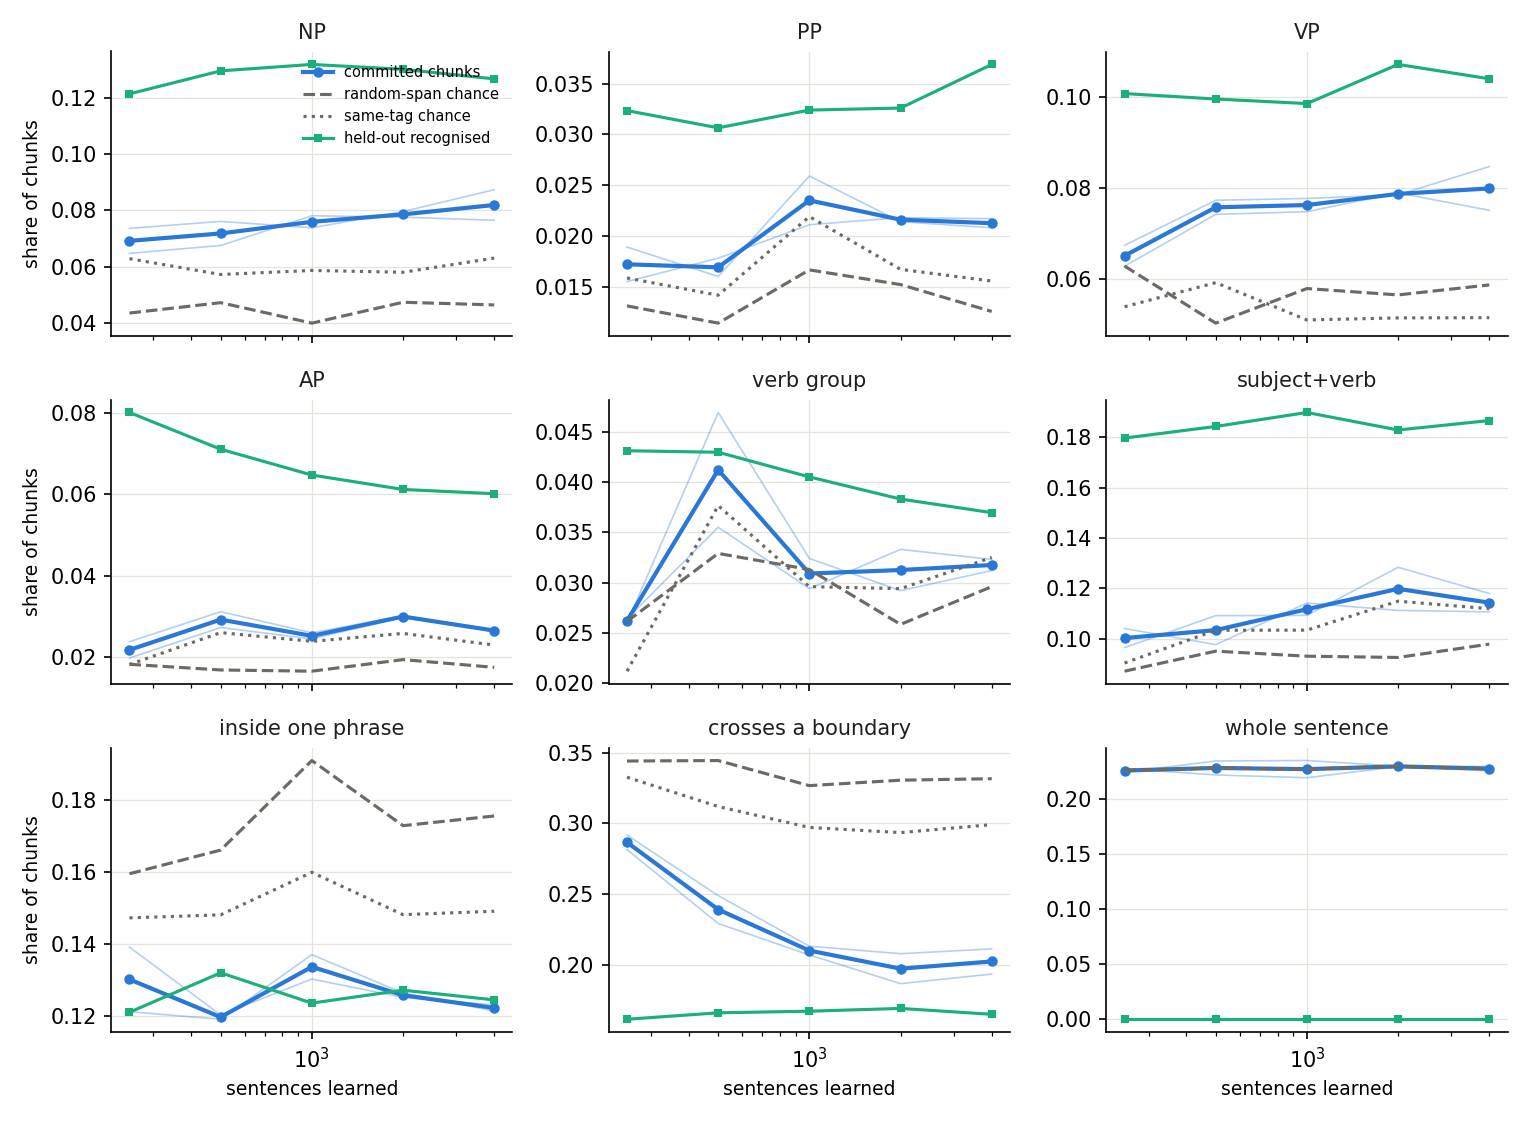
\includegraphics[width=0.8\textwidth]{figures/story_chunks_curves}
\caption{Share of committed chunks of each type against training sentences on TinyStories (blue; thin lines are seeds), where a committed chunk is a composite of the tree chosen during learning that the system stored as a record.
Dashed lines show random-group chance and dotted lines show chance for groups that start on a word of the same tag. The green line shows the share of recognized groups in held-out sentences.
Types come from the NLTK reference, and ``crosses a boundary'' marks chunks that straddle a reference phrase. The share of boundary-crossing chunks falls with experience.}
\label{fig:chunkcurves}
\end{figure}

\begin{figure}[!t]
\centering
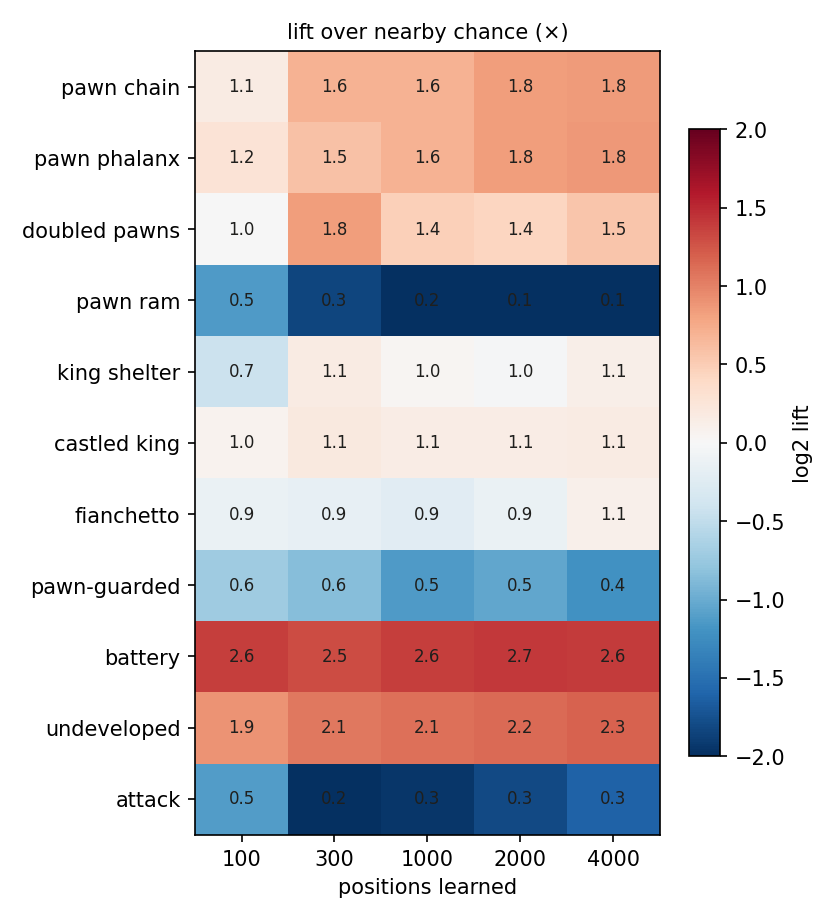
\includegraphics[width=0.45\textwidth]{figures/chess_ideas_lift}
\caption{Lift over nearby-piece chance of the share of recognized chunks that carry each chess idea, five-seed mean, positions from Lichess games.
Chance labels groups of nearby pieces of the same size as the chunks, so a lift above one means that memory prefers the idea.}
\label{fig:chessideas}
\end{figure}

\begin{figure}[!t]
\centering
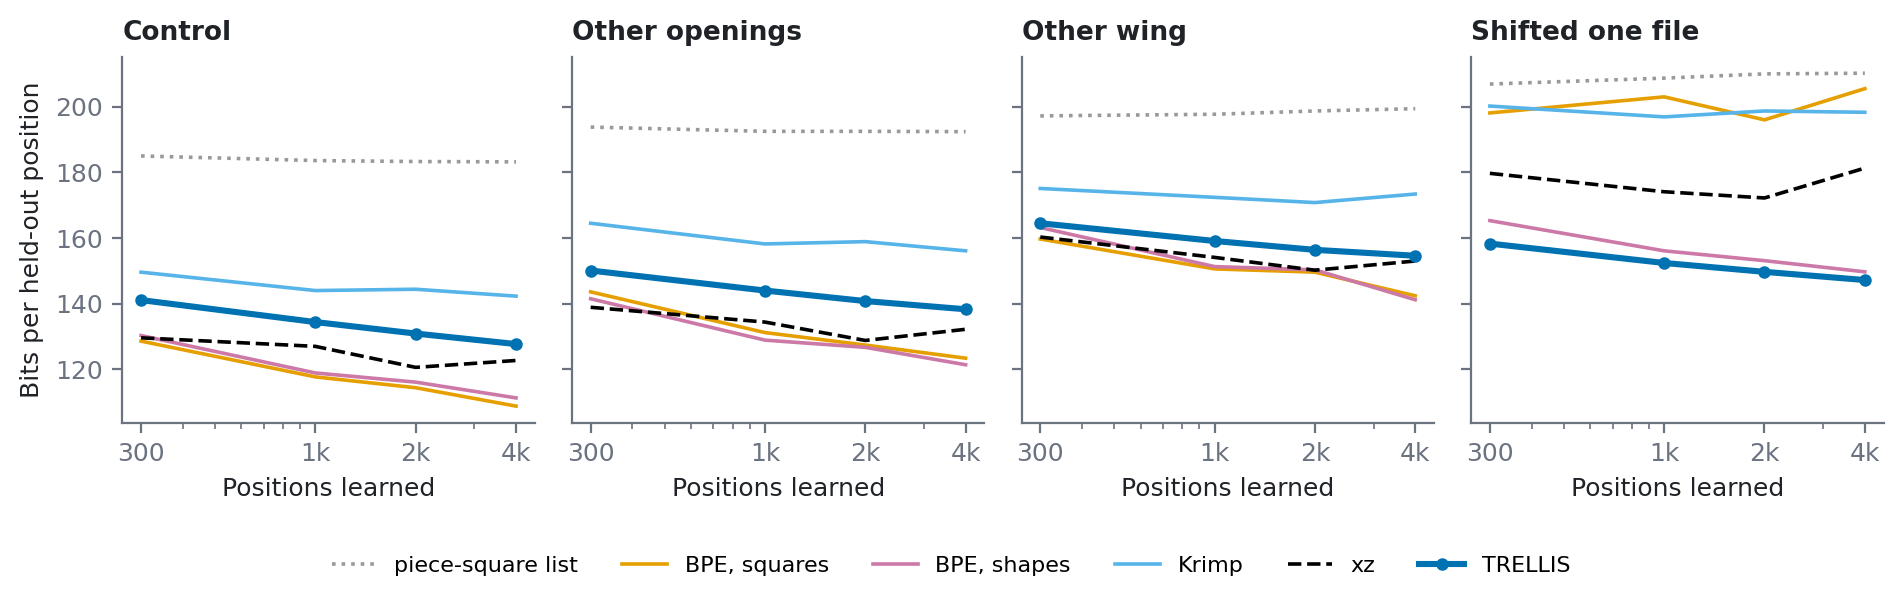
\includegraphics[width=\textwidth]{figures/chess_chunkers}
\caption{Bits per held-out Lichess position against positions learned (300 to 4,000) for \trellis{} and the comparison coders, on four test sets: control, other openings, other wing, and positions shifted one file (seed 13, model cost not charged).
The \trellis{} curve is the better of its offsets-only and offsets-plus-squares variants in each panel.
Its shifted panel therefore uses a variant that the standard chess configuration C5 does not allow, and the main paper gives both values.}
\label{fig:chesscompress}
\end{figure}

\begin{table}[h]
\caption{First-trial recall of pieces on Lichess middle-game, end-game, and random positions after \trellis{} learned 300, 1,000, and 4,000 positions (mean over three seeds, 13, 17, and 19, with ten simulated subjects each), with seven and four chunk slots,
next to the recall that Chase and Simon (1973) report for people as beginner, class A player, and master. Random positions average the middle-game and end-game random sets (4.3 and 4.1 at 300 positions with seven slots).
The human values for random positions come from a single master, class A player, and beginner as reported in the source.}
\label{tab:cs}
\begin{center}
\small
\begin{tabular}{llccc}
\toprule
Positions & Memory & 300 / beginner & 1,000 / class A & 4,000 / master \\
\midrule
Middle game & \trellis{}, 7 slots & 7.2 & 9.7 & 12.9 \\
 & \trellis{}, 4 slots & 4.3 & 6.7 & 9.5 \\
 & People & 4 & 8 & 16 \\
End game & \trellis{}, 7 slots & 5.8 & 6.7 & 7.4 \\
 & \trellis{}, 4 slots & 3.4 & 3.9 & 4.5 \\
 & People & 4 & 7 & 8 \\
Random & \trellis{}, 7 slots & 4.2 & 5.5 & 6.0 \\
 & \trellis{}, 4 slots & 2.2 & 2.8 & 3.2 \\
 & People & 3.0 & 2.5 & 2.0 \\
\bottomrule
\end{tabular}
\end{center}
\end{table}

\begin{table}[h]
\caption{Chess move quality for 200 Lichess positions at ply 30 after \trellis{} learned 1,000 positions (seed 13). The legal-move rows choose among legal moves; the displacement rows add 120 random piece displacements per position.
Sound moves lose less than two pawns of material by a fixed capture search. Real game continuations are sound .983 of the time on 300 validation positions, random legal moves .697, and worst legal moves .033.
Binomial uncertainty on 200 positions is about $\pm.065$.}
\label{tab:chessmoves}
\begin{center}
\small
\begin{tabular}{lccc}
\toprule
Candidates and choice & Sound & Legal but losing & Illegal \\
\midrule
Legal moves, best recognized & .625 & .375 & 0 \\
Legal moves, uniform random & .655 & .345 & 0 \\
Any displacement, best recognized & .125 & .105 & .770 \\
\bottomrule
\end{tabular}
\end{center}
\end{table}

When the candidates include random piece displacements, the model receives no rules, and about three quarters of the candidates are illegal. The best-recognized pick is illegal .77 of the time against .70 for a random pick.
The material criterion catches hung pieces and lost exchanges and misses positional sense.

\section{Regimes}

\paragraph{Judge controls.} Table~\ref{tab:judge} gives the pass rates of the ensemble on control sentences built from held-out stories.

\begin{table}[h]
\caption{Share of control sentences passed by the Qwen3-8B and phi-4 ensemble on the syntax and meaning questions (test half, 150 sentences per class, built from held-out TinyStories sentences).
The content-word swap here is the ensemble study's own, built with animacy and emotion flips and listed verb frames, and differs from the tag-based swap of the broken-sentence studies.}
\label{tab:judge}
\begin{center}
\small
\begin{tabular}{llcc}
\toprule
Control class & Example & Syntax pass & Meaning pass \\
\midrule
Real & the fish was not happy anymore & 1.00 & .95 \\
Content words swapped & the hard door looked hard & .88 & .13 \\
Two adjacent words swapped & little the bird looked sad & .13 & .06 \\
Agreement error & they is not friends anymore & .04 & .15 \\
Scrambled & not anymore was happy the fish & .02 & .00 \\
\bottomrule
\end{tabular}
\end{center}
\end{table}

\paragraph{Dial.} Table~\ref{tab:dial} gives the regime shares at each abstraction level for the three runs behind Figure 8 of the main paper.
The leaf row at generation temperature 1 matches the temperature of the class levels, and the leaf row at temperature .7 is the best leaf setting.
Table~\ref{tab:law} normalizes by the temperature-1 leaf. Normalizing by the temperature-.7 leaf instead gives a meaningless share of .21 to .23 at the leaf, and the ordering across levels stays the same.
As a null for abstraction along the word taxonomy, a class-free swap replaces every word outside the 50 most frequent types by a random type, starting from meaningful sentences of the temperature-.7 leaf.
It leaves a meaningless share of grammatical output of .32, .45, and .43 on the three runs (syntax-only .078, .099, and .086 against meaningful .167, .122, and .113). Random damage also raises the share, so the ordering alone does not distinguish abstraction along the taxonomy from damage in general.

\begin{table}[h]
\caption{Share of generated TinyStories sentences in each regime (judge 2; configuration C6) as the generator's context moves from exact words (leaf) to one class (root), seed 13 after 1,000 and 4,000 sentences and seed 17 after 4,000.
Meaningful passes syntax and meaning, syntax-only passes syntax alone, and nonsense fails syntax. Both leaf rows use the pair gate. The temperature-.7 leaf row is the setting with the highest meaningful share (window 7 at 1,000 sentences and window 5 at 4,000 sentences).
All other rows use generation temperature 1. Class levels use a word taxonomy that Cobweb builds from each word's neighbors and the function words beside it.
They also use a class-level pair gate, which admits a pair when memory stored some adjacent pair from the same two classes. Entries are meaningful / syntax-only / nonsense.}
\label{tab:dial}
\begin{center}
\footnotesize
\begin{tabular}{lccc}
\toprule
Setting & 1,000, seed 13 & 4,000, seed 13 & 4,000, seed 17 \\
\midrule
Leaf, temperature 1 & .558 / .206 / .235 & .580 / .193 / .228 & .541 / .218 / .241 \\
Leaf, temperature .7 & .630 / .170 / .201 & .634 / .176 / .190 & .621 / .182 / .197 \\
Class level $b=7$ & .331 / .255 / .415 & .293 / .211 / .497 & .323 / .265 / .412 \\
Class level $b=6$ & .197 / .208 / .595 & .180 / .161 / .658 & .201 / .225 / .574 \\
Class level $b=4$ & .107 / .140 / .753 & .087 / .116 / .797 & .116 / .157 / .727 \\
Root (one class) & .034 / .095 / .871 & .029 / .082 / .889 & .033 / .083 / .885 \\
\bottomrule
\end{tabular}
\end{center}
\end{table}

\begin{table}[h]
\caption{Pass rates and the meaningless share by abstraction level (judge 2, configuration C6; the three runs of Table~\ref{tab:dial}).
Syntax pass is the share of generated sentences that are meaningful or syntax-only, and meaning pass is the share that are meaningful. Retained values divide by the temperature-1 leaf value of the same run.
Entries give the range over the three runs.}
\label{tab:law}
\begin{center}
\small
\begin{tabular}{lccc}
\toprule
Level & Syntax pass retained & Meaning pass retained & Meaningless share of grammatical \\
\midrule
Leaf & 1.00 & 1.00 & .25 -- .29 \\
$b=7$ & .65 -- .77 & .51 -- .60 & .42 -- .45 \\
$b=6$ & .44 -- .56 & .31 -- .37 & .47 -- .53 \\
$b=4$ & .26 -- .36 & .15 -- .21 & .57 -- .58 \\
Root & .14 -- .17 & .05 -- .06 & .72 -- .74 \\
\bottomrule
\end{tabular}
\end{center}
\end{table}

\paragraph{Oracles for the middle regime.} The largest syntax-only share over every setting, seed, and size is .265, against a target of .5. We looked for the cause with oracles that need no model, and two protocols appear.
Protocol A takes the meaningful sentences of the best generator and replaces every word outside the 50 most frequent word types with another type of the same class, and the judge scores the result ($K=50$).
Under protocol A, classes from the learned word taxonomy leave at most .208 of the sentences syntax-only at 1,000 sentences, and .181 and .203 at 4,000 sentences on two seeds. Part-of-speech classes give .199, .211, and .217, so the generators already sit at the level of this oracle.
Protocol B protects no frequent types ($K=0$) and swaps only nouns, verbs, and adjectives. Under it, an oracle that swaps within exact morphosyntactic cells (tense, number, verb frame) reaches .45, .50, and .52 syntax-only on three runs, and the same cells with the 50 most frequent types protected give .31 to .34 (Table~\ref{tab:oracle}).
Protocol B supersedes the verdict of protocol A that substitution itself caps the regime: a clean syntax-only output exists when classes are fine and every content word is replaced.
Swapping across a coarse class breaks agreement and verb frames, which the judge treats as syntax failures, and about half of the part-of-speech swaps lose syntax for that reason.
Protocol A's ceiling does not rise with more text, because the same 250-word vocabulary at 4,000 sentences leaves it at .18 to .22.
Class sources that need no labels fall short of the cell oracle under protocol B. The levels of the learned word taxonomy mix tags and frames, so only .4 to .5 of the members of a class share a morphosyntactic signature.
A later test added each word's own ending (its last one to three characters) and the nearest function words to the left and right as features of the word taxonomy. It also cut classes by size as well as by depth.
Every tree-class oracle stayed at a syntax-only share of .15 to .395 (typically .30 to .38), and class purity stayed at .4 to .58, so no generator here uses these classes.
We searched for a level of the context taxonomy at which the slots of committed word occurrences are pure in part of speech (at least .8) and varied (at least 3 bits of filler entropy), and found none. Purity reaches .8 only at the leaf, where filler entropy is .03 bits.
A feature that sees a verb's complement, or a tagging pass, would be a different mechanism, and no experiment here tests one.

\begin{table}[h]
\caption{Share of oracle sentences that are syntax-only under the two oracle protocols (judge 2). Both start from the meaningful sentences of the pair-gated word generator and swap words within a class.
Protocol A protects the 50 most frequent word types ($K=50$) and swaps every other word. Protocol B protects none ($K=0$) and swaps nouns, verbs, and adjectives.
Values are for 1,000 sentences on seed 13 and 4,000 sentences on seeds 13 and 17.}
\label{tab:oracle}
\begin{center}
\small
\begin{tabular}{llccc}
\toprule
Protocol & Classes & 1,000, s13 & 4,000, s13 & 4,000, s17 \\
\midrule
A ($K=50$) & learned word taxonomy & .208 & .181 & .203 \\
A ($K=50$) & part of speech & .199 & .211 & .217 \\
A ($K=50$) & morphosyntactic cells & .31 & .33 & .34 \\
B ($K=0$) & morphosyntactic cells & .45 & .50 & .52 \\
B ($K=0$) & learned word taxonomy, best cell & -- & .349 & .395 \\
\bottomrule
\end{tabular}
\end{center}
\end{table}

\paragraph{Context length and context abstraction.} The reach $W'$ sets the number of left-context words that the generator reads, and abstracting the context replaces the exact words in its window by classes of the word taxonomy at level $b$ while the emitted word stays exact (configuration C9, seed 13, 1,000 sentences, window 5, judge 2).
Table~\ref{tab:ctx} gives the regime shares. With exact words, context length is a clean dial between the meaningful and nonsense ends. The meaningful share is .28 at $W'=1$, .61 at 2, .68 at 3, and .60 at 5, and a reach of zero yields .85 nonsense and .07 meaningful.
Abstracting the context moves mass from meaningful to nonsense. At $W'=3$ the meaningful share falls from .68 at the leaf to .57 at $b=4$ and to .41 to .48 at the root, and the nonsense share rises from .14 to .20 and to .28 to .37.
The syntax-only share never exceeds .245 in any of the 36 cells, and abstracting the function words of the context as well leaves the same limit. The word-level pair gate keeps every adjacent pair a stored bigram, so local syntax holds in every cell, and abstraction removes the long-range selection that keeps sentences sensible.
The middle cells yield syntax-only sentences only when a word repeats or the object is odd, in about one draw in five. The study ran at one size and one seed, because it stopped before 4,000 sentences.

\begin{table}[h]
\caption{Regime shares (meaningful / syntax-only / nonsense; judge 2, configuration C9, seed 13, 1,000 sentences, window 5, generation temperature 1, pair gate on) by context reach $W'$ and context abstraction level $b$.
Leaf means exact context words, and the root class acts as a wildcard. $K$ is the number of most frequent word types kept exact. Values are rounded.
The table shows 16 of the 36 cells (the $b=7$ and $b=6$ rows are omitted), and the largest syntax-only share over all 36 is .245.}
\label{tab:ctx}
\begin{center}
\footnotesize
\begin{tabular}{lccccc}
\toprule
Context & $W'=0$ & $W'=1$ & $W'=2$ & $W'=3$ & $W'=5$ \\
\midrule
Leaf, $K=25$ & .07 / .09 / .85 & .28 / .20 / .53 & .61 / .21 / .19 & .68 / .18 / .14 & .60 / .17 / .23 \\
$b=4$, $K=50$ & -- & .30 / .20 / .51 & .46 / .25 / .29 & .57 / .23 / .20 & .55 / .23 / .23 \\
Root, $K=25$ & -- & .23 / .18 / .60 & .36 / .19 / .45 & .41 / .22 / .37 & .42 / .23 / .35 \\
Root, $K=50$ & -- & .29 / .16 / .55 & .42 / .21 / .37 & .48 / .24 / .28 & .46 / .24 / .30 \\
\bottomrule
\end{tabular}
\end{center}
\end{table}

\paragraph{Chess regimes.} Table~\ref{tab:chesslaw} gives every route of the chess study (configuration C11, two seeds, 4,000 positions learned, 500 boards per cell for the content-dial rows and 600 for the others).
A board is legal by the rules of chess (python-chess, White to move). A piece-square classifier calibrated on real positions decides realism, and we call a legal board that the classifier accepts R-real, a legal board that it rejects R-legal, and an illegal board R-non.
Real held-out positions are R-real in .957 of cases, random legal boards are R-legal in .97 of cases, and random illegal boards are R-non always.
Drawing positions from the chunk and concept distributions alone gives R-real of .085 at the leaf and .006 at the root. R-legal never exceeds .015, because the whole-board counts (one king per side, at most eight pawns) belong to no unit-level distribution.
Adding a stored piece-count profile lifts R-real to at most .54 and R-legal to at most .098.
Parsing a held-out position and regenerating its chunks keeps the real structure at the leaf (R-real .76). Replacing chunk contents at any higher concept level gives nonsense (R-non .72 at level 1 and about .94 from level 2 up), because the replacement chunks bring their own kings and pawns. The legal-unrealistic regime stays at or below .058 in these routes.

\begin{table}[h]
\caption{Chess regime shares (R-real / R-legal / R-non) after 4,000 learned positions, mean of two seeds, with the same judge for every row (legality by python-chess, realism by a piece-square classifier).
Where-file and where-rank redraw one coordinate of the anchor (the reference square) of each parsed chunk, where-both redraws both, and what replaces the chunk's pieces by a stored instance. Root draws from any anchor in the tree, and the leaf draws from anchors stored under the chunk's own concept.
Identity replaces the pieces of every chunk as well, and level $k$ is the concept level at which the draw is made. The content-dial and parse-and-regenerate rows are earlier routes from the same learner.}
\label{tab:chesslaw}
\begin{center}
\footnotesize
\begin{tabular}{lccc}
\toprule
Setting & R-real & R-legal & R-non \\
\midrule
Real board through the parser & .945 & .055 & .000 \\
Content dial only, leaf / root & .085 / .006 & .000 / .005 & .915 / .989 \\
Parse and regenerate, leaf / level 2 & .762 / .043 & .051 / .019 & .188 / .938 \\
Where-file, leaf & .890 & .056 & .054 \\
Where-file, level 1 & .790 & .139 & .073 \\
Where-file, level 2 & .738 & .184 & .077 \\
Where-file, root & .681 & .233 & .085 \\
Where-rank, leaf & .829 & .053 & .118 \\
Where-rank, level 2 & .480 & .091 & .428 \\
Where-rank, root & .193 & .137 & .671 \\
Where-both, root & .080 & .137 & .782 \\
Where-file and what, root & .003 & .014 & .984 \\
Where-both and what, root & .002 & .009 & .990 \\
Piece list, counts off / on & .099 / .504 & .003 / .006 & .898 / .490 \\
\bottomrule
\end{tabular}
\end{center}
\end{table}

\section{Items Moved from the Main Paper}

\paragraph{Confirmation seeds.} Table~\ref{tab:genconf} gives the fair count of the four confirmation seeds (29, 31, 37, and 41), which chose no setting. It complements Table 4 of the main paper, which pools all eight seeds.

\begin{table}[h]
\caption{Fair count on TinyStories under judge 2 for the confirmation seeds 29, 31, 37, and 41 (configuration C1; per-seed values rounded to three digits). Paired differences give the mean, the 95\% $t$ interval on four seeds, and the seeds won. The Qwen2.5-3B judge chose the settings.}
\label{tab:genconf}
\begin{center}
\footnotesize
\begin{tabular}{rcccll}
\toprule
$n$ & \trellis{} & LSTM & GPT & \trellis{} $-$ LSTM & \trellis{} $-$ GPT \\
\midrule
\multicolumn{6}{l}{\textit{Syntax pass}} \\
250   & .308 & .287 & .281 & +.021 [$-$.016, +.059], 3/4 & +.027 [+.010, +.044], 4/4 \\
500   & .366 & .378 & .362 & $-$.012 [$-$.024, +.001], 0/4 & +.004 [$-$.056, +.064], 2/4 \\
1,000 & .399 & .413 & .427 & $-$.014 [$-$.072, +.043], 1/4 & $-$.028 [$-$.059, +.003], 0/4 \\
\multicolumn{6}{l}{\textit{Syntax and meaning pass}} \\
250   & .191 & .176 & .162 & +.015 [$-$.010, +.040], 3/4 & +.029 [$-$.011, +.070], 4/4 \\
500   & .220 & .241 & .213 & $-$.022 [$-$.039, $-$.005], 0/4 & +.006 [$-$.026, +.039], 3/4 \\
1,000 & .254 & .275 & .275 & $-$.020 [$-$.059, +.018], 1/4 & $-$.021 [$-$.055, +.013], 0/4 \\
\bottomrule
\end{tabular}
\end{center}
\end{table}

\paragraph{Parse score and generator score.} Figure~\ref{fig:parsecurve} gives the share of broken held-out sentences that each score accepts as training grows (configuration C4, set C; Tables~\ref{tab:parse} and~\ref{tab:auc} give the values and the AUC).


\begin{figure}[!t]
\centering
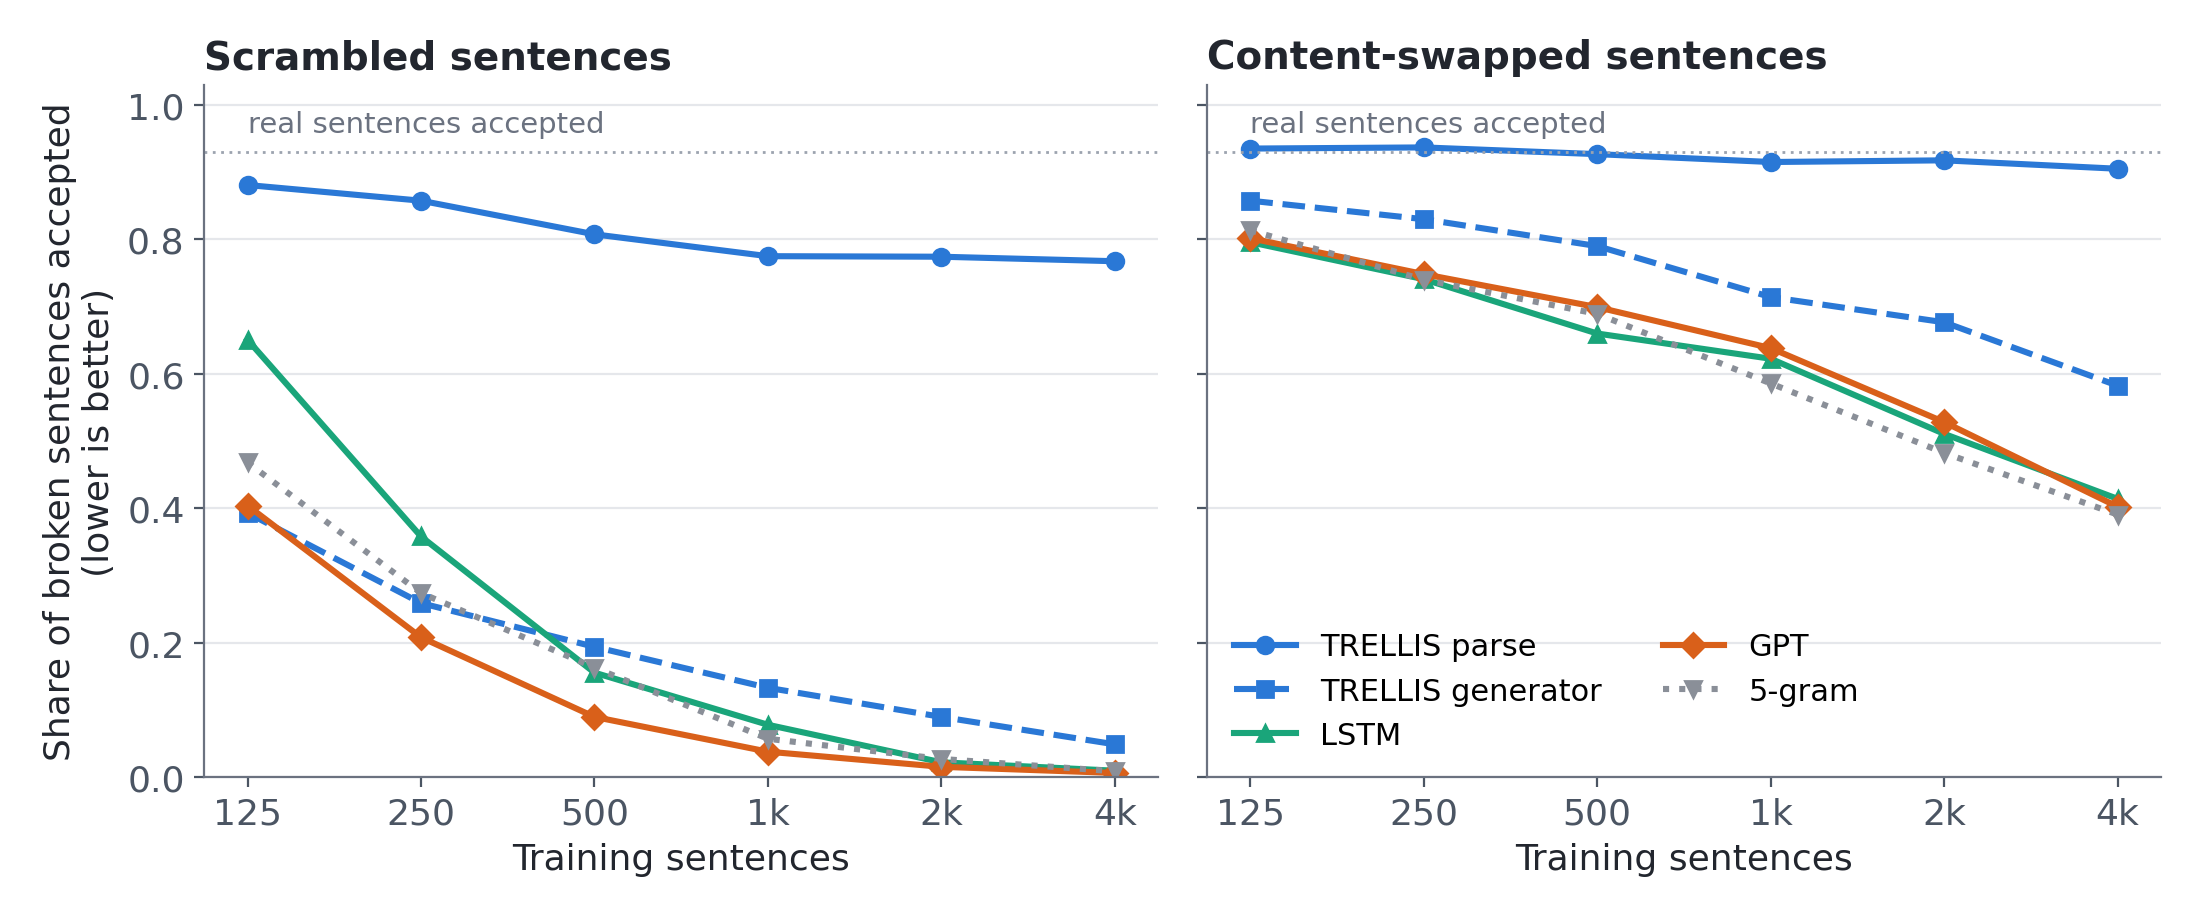
\includegraphics[width=0.7\textwidth]{figures/parse_success_curve}
\caption{Share of broken held-out TinyStories sentences accepted by each score against training sentences (configuration C4, set C, four seeds). The threshold accepts 90\% of real calibration sentences, so lower is better.
Parse and generator scores come from \trellis{}, and the LSTM and GPT train on the same sentences.}
\label{fig:parsecurve}
\end{figure}

\paragraph{Code length in language.} Figure~\ref{fig:bits} gives the held-out code length against training sentences for \trellis{} and the comparison coders, as the main paper describes.


\begin{figure}[!t]
\centering
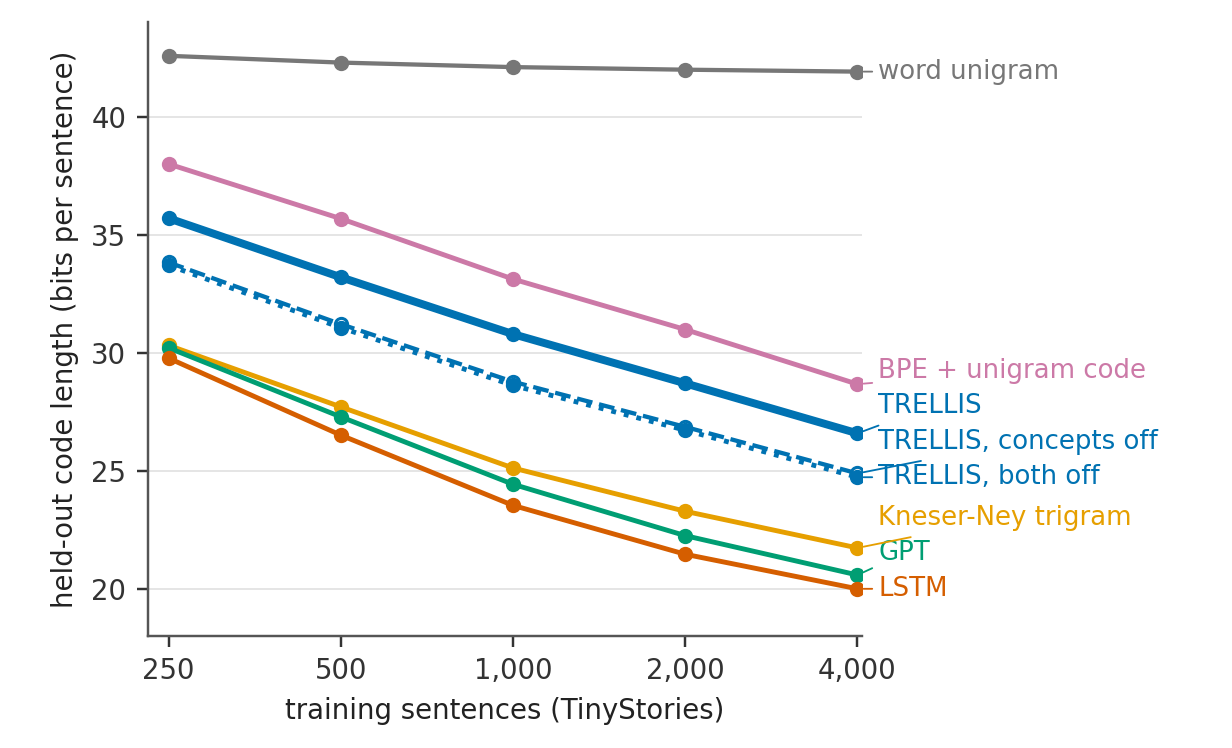
\includegraphics[width=0.6\textwidth]{figures/language_bits_curve}
\caption{Held-out code length in bits per sentence against training sentences on TinyStories (first 1,000 held-out sentences, seeds 13 and 17 averaged; model cost not charged). The uniform code costs 51.4 bits.
\trellis{} is the generator's code with a uniform escape (configuration C8). The dashed line removes the concepts from the generator's reads, and the dotted line removes the chunks and the concepts.
Removing only the chunks overlaps the solid \trellis{} line and is not drawn. The n-gram is a Kneser-Ney trigram.}
\label{fig:bits}
\end{figure}

\paragraph{Removal controls in language.} Table~\ref{tab:ablation} removes the parts of the generator at 1,000 sentences, as the main paper describes.

\begin{table}[h]
\caption{Removal controls on TinyStories after 1,000 sentences (seeds 13 and 17, configuration C8). Code length is bits per held-out sentence. Fair counts use judge 2 at temperature 2.0 and omit the unstored-trigram requirement, so they differ from Table 4 of the main paper.
Content swap accepted is the share of content-swapped sentences that the generator score accepts at the threshold that accepts 90\% of real sentences (lower is better).
Chunks off stores no composite. Concepts off reads every record at its own leaf, with back-off to the root. Both off combines the two.}
\label{tab:ablation}
\begin{center}
\small
\begin{tabular}{lcccc}
\toprule
Variant & Code length & Fair syntax & Fair syntax and meaning & Content swap accepted \\
\midrule
Full & 30.8 & .539 & .363 & .708 \\
Chunks off & 30.8 & .520 & .347 & .707 \\
Concepts off & 28.8 & .496 & .309 & .573 \\
Both off & 28.6 & .512 & .311 & .575 \\
\bottomrule
\end{tabular}
\end{center}
\end{table}


\paragraph{Removal controls in chess.} Table~\ref{tab:chess-abl} gives the removal controls of the chess study at 4,000 positions.

\begin{table}[h]
\caption{Removal controls in chess after 4,000 learned Lichess positions (configuration C10, mean of seeds 13, 17, and 19; model cost not charged). Top: bits to code 1,000 held-out positions per set; the piece-square list codes each piece independently from the frequencies of its square.
Bottom: first-trial recall of pieces on middle-game, end-game, and random positions with seven chunk slots (ten simulated subjects per seed, each recalling its own random draw of positions). Full-system code lengths are three-seed means and differ slightly from the seed-13 values in Table 5 of the main paper. Concepts-off recall is zero by construction.}
\label{tab:chess-abl}
\begin{center}
\small
\begin{tabular}{lcccc}
\toprule
Bits per position & Control & Other openings & Other wing & Shifted \\
\midrule
Full system & 129.2 & 137.5 & 153.4 & 151.5 \\
Concepts off & 129.9 & 138.2 & 153.8 & 152.1 \\
Chunks off & 183.3 & 191.9 & 200.7 & 210.7 \\
Piece-square list & 181.9 & 190.4 & 198.3 & 208.9 \\
\midrule
Recall, seven slots & Middle game & End game & Random middle & Random end \\
\midrule
Full system & 12.9 & 7.4 & 5.9 & 6.1 \\
Chunks off & 7.0 & 6.9 & 6.4 & 6.3 \\
Concepts off & 0.0 & 0.0 & 0.0 & 0.0 \\
\bottomrule
\end{tabular}
\end{center}
\end{table}

\paragraph{Recall across experience.} Figure~\ref{fig:cscurve} gives first-trial recall against positions learned, as the main paper describes.

\begin{figure}[!t]
\centering
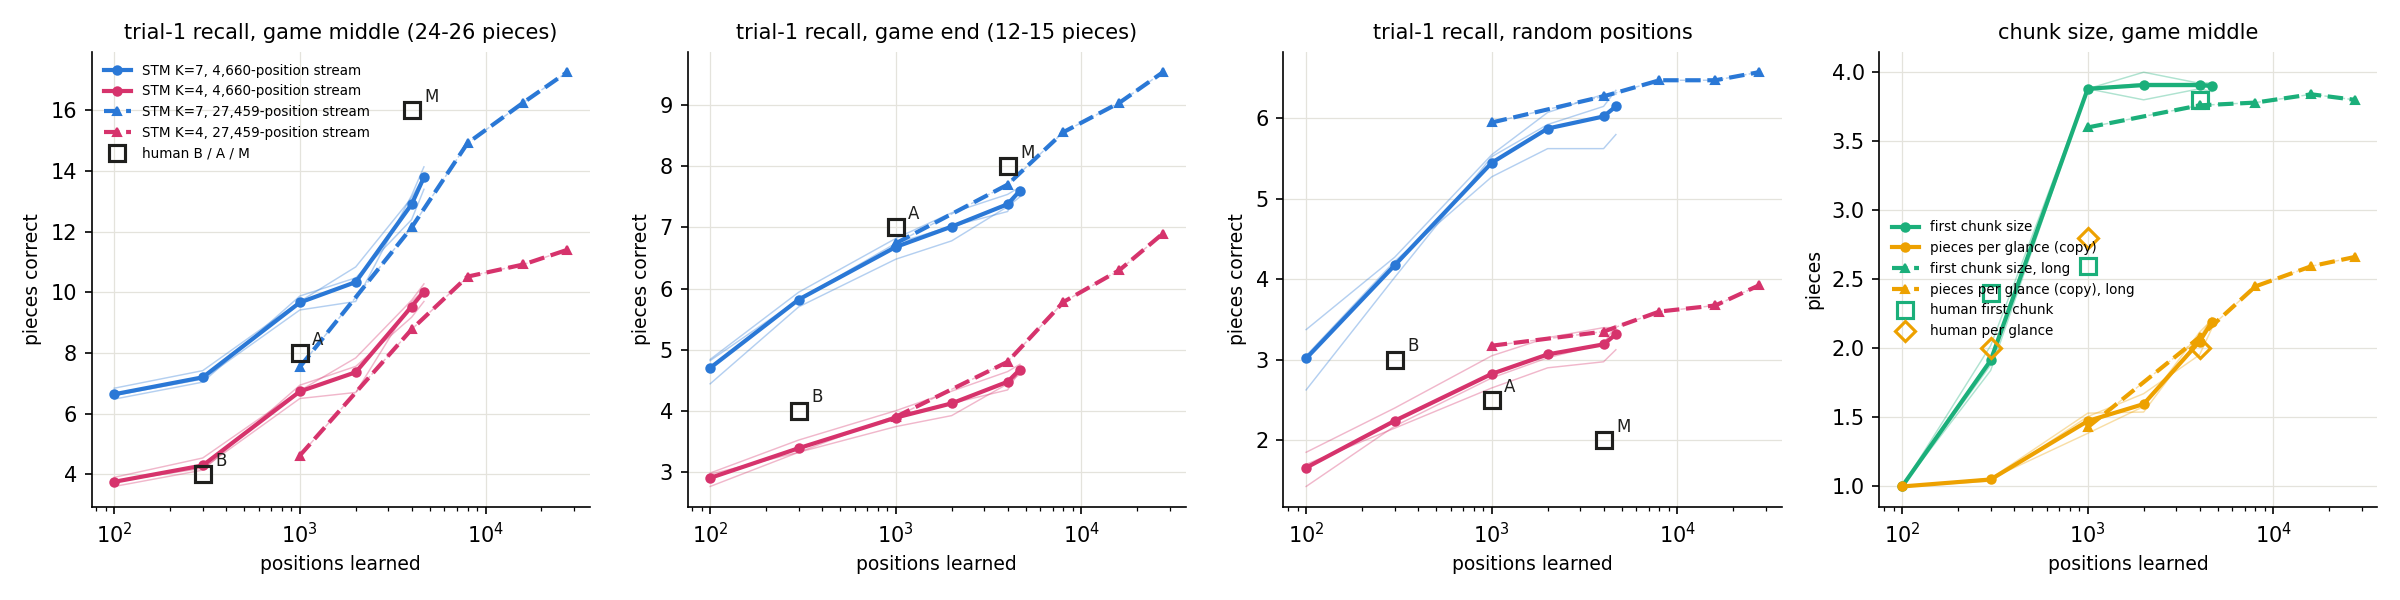
\includegraphics[width=\textwidth]{figures/chess_cs1973_curve}
\caption{Recall of Lichess middle-game, end-game, and random positions against positions learned (solid lines: 100 to 4,660 positions, three seeds; dashed lines: 1,000 to 27,459 positions, the long stream), with seven and four chunk slots, next to people's recall (black squares: beginner B, class A player A, master M).
The right panel shows the size of the first chunk and the pieces per glance, the pieces placed after one look at the board while a subject copies a board that stays in view (Chase and Simon's copy task). Thin lines are single seeds.}
\label{fig:cscurve}
\end{figure}

\paragraph{File symmetry of the chess judge.} The realism judge of the chess regime study (tau = .702) is a logistic regression on piece-square indicators, piece counts, pawns per file, and material. We moved the 1,000 real held-out positions of its validation set sideways and kept the legal results. The moves were every shift of one or two files that keeps all pieces on the board and the mirror image from the a-file to the h-file. Table~\ref{tab:filesym} gives the share scored real.

\begin{table}[h]
\caption{Share of file-shifted real held-out positions that the chess realism judge scores real (all results legal; shifts fit only positions without pieces near both edges). Random legal boards score real in .03 of cases.}
\label{tab:filesym}
\begin{center}
\small
\begin{tabular}{lccc}
\toprule
Transform & Positions & Scored real & Share \\
\midrule
None & 1,000 & 957 & .957 \\
Mirror a to h & 1,000 & 789 & .789 \\
Shift +1 file & 26 & 16 & .615 \\
Shift $-$1 file & 53 & 38 & .717 \\
Shift +2 files & 4 & 2 & .500 \\
Shift $-$2 files & 13 & 5 & .385 \\
\bottomrule
\end{tabular}
\end{center}
\end{table}

\end{document}
